\chapter{Implementierung}

\section{Die Spieleverwaltung}
\sectionauthor{\frank}

Ziel eines derartigen Frameworks ist, dieses möglichst modular \unsure{Ist das
das Ziel?} zu entwickeln. Dazu gehört auch, es zu ermöglichen, Spiele einfach
und dynamisch hinzufügen zu können. Sicher könnte man dessen benötigten Klassen
erstellen und anschließend an irgendeiner Stelle in die App hardcoden. Doch wir
wollten all das, was zu diesem Prozess gehört vereinfachen, und damit
flüssiger, angenehmer und vor allem modularer gestalten. Dadurch wird auch das
nachträgliche Ändern oder Löschen von Spielen trivial. Außerdem wird so der Weg
für zukünftige Automatisierung -- wie beispielsweise Spielständen -- geebnet.

\subsection{Deklaration von Spielen}

Die Deklaration und Deklaration von Spiele-Metadaten erfolgt strukturiert in
einer XML-Datei, \emph{games.xml}, welche durch eine \textbf{Document Type
Definition} semantisch abgesichert ist. So wird gewährleistet, dass die Spiele
im passenden Format vorliegen, und so entsprechend weiterverarbeitet werden
können. Die Datei erlaubt außerdem die Zuordnung in selbst gewählte
Spiele-Kategorien, wie zum Beispiel \emph{Kartenspiele} oder \emph{Brettspiele}.

Hier ist ein Auszug, der die verwendete DTD zeigt:

\begin{lstlisting}
<!DOCTYPE games [
    <!ELEMENT games (category*)>
    <!ELEMENT category (game*)>
    <!ATTLIST category id ID #REQUIRED>
    <!ATTLIST category title CDATA #REQUIRED>
    <!ATTLIST category icon CDATA #REQUIRED>
    <!ELEMENT game EMPTY>
    <!ATTLIST game title CDATA #REQUIRED>
    <!ATTLIST game description CDATA #REQUIRED>
    <!ATTLIST game icon CDATA #REQUIRED>
    <!ATTLIST game rules CDATA #REQUIRED>
    <!ATTLIST game tag CDATA #IMPLIED>
    <!ATTLIST game activity CDATA #REQUIRED>
]>
\end{lstlisting}

\subsubsection{Kategorien}

Wie man daraus ablesen kann, können unter dem Root-Element \code{games} beliebig
viele Kategorien hinzugefügt werden. Eine solche Kategorie wird beschrieben
durch drei verpflichtende Attribute. \code{id} ist eindeutig im gesamten
Deklarationsbereich, also der Datei zu wählen. Sie wird später weiter verwendet,
um eine Kategorie eindeutig zu Identifizierung und wiederzufinden.  \code{title}
ist die Bezeichnung dieser Kategorie, bei welcher es möglich ist Text aus der
\emph{strings.xml}-Datei zu referenzieren. Solche Referenzierungen werden in der
Form \code{"@strings/ref"} angegeben, wobei \code{ref} für den entsprechenden
Identifikator steht. Außerdem ist noch ein Icon anzugeben, das später
beispielsweise im Navigation Drawer zu finden ist. Hier ist ebenfalls die
Referenzierung einer Resource möglich.

\subsubsection{Spiele}
\label{sssec:games}

Spiele werden analog unter den Kategorien angegeben. Sie besitzen jedoch
unterschiedliche Attribute. \code{title} und \code{icon} stimmen mit der
Funktionalität dessen \unsure{dessen?} einer Kategorie überein. Ihre Werte kann
man beispielsweise in der Spieleliste oder in der Android-Actionbar sehen.
Zusätzlich sind die beschreibenden Attribute \code{description}, \code{rules}
hinzuzufügen. \code{activity} bestimmt später in der laufenden Anwendung, welche
Aktivität gestartet wird, wenn man auf das Spiel in der Liste klickt. Die
Aktivität muss im Package \emph{activity} unter \emph{view} im Root-Package
liegen, um gestartet werden zu können. Sie wird mit ihrem Ort unterhalb dieses
Paketes angegeben, zum Beispiel \emph{``Chess''}. Das letzte Attribut \code{tag}
ist zur weiteren Eigenschaftsbestimmung eines Spiels gedacht und kann später in
der Aktiviät selbst abgefragt werden. Mit diesem Tag ist es möglich weitere
Varianten eines Spieles anzulegen, ohne dafür neue Aktivitäten / Klassen
anfertigen zu müssen. Es ist darüberhinaus gegeben, mehrere Tags festzulegen,
diese werden durch \emph{|} getrennt. Im Falle eines 2-Spieler Schach-960's,
lautet dieser \code{``aiGame|chess960''}.

\subsubsection{Beispiel}

Eine Datei mit genauer einer Kategorie und einem Spiel würde also so aussehen:

\begin{lstlisting}
<?xml version="1.0" encoding="utf-8"?>
<games>

    <category
        id="boardgames"
        title="@string/boardgames"
        icon="@drawable/icon_checkerboard">

        <game
            title="@string/game_chess_title"
            description="@string/game_chess_player_vs_ai"
            icon="@mipmap/ic_launcher"
            rules="@string/game_chess_rules"
            tag="aiGame"
            activity="Chess" />

    </category>

</games>
\end{lstlisting}

Die \textbf{DTD} wurde aus Platzgründen weggelassen.

\subsection{Die Spiele-Klasse}

Passend zu der Beschreibung eines Spiels in der XML-Datei gibt es die Klasse
\code{Game}. In ihr befinden sich die äquivalenten Attribute zur Markup-Datei.
Außerdem besitzt diese Klasse eine Instanzmethode \code{boolean
isTaggedWith(String tag)}, welche abfragt, ob das übergebene Argument Teil des
Tags ist. So kann eine Spieleaktivität ganz ohne Umschweife die Eigenschaften
des zugehörigen Elements aus der Deklarationsdatei abfragen, um bestimmte
Abfolgen des Spielverlaufes zu verändern. Siehe \autoref{sssec:games}.

\subsection{Der Spielemanager}

\includegraphics{resources/tobecontinued}

\change{Bessere Graphik und Caption}
\begin{figure}[h]
	\centering
	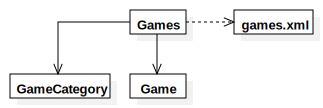
\includegraphics{resources/gamemanager/gamemanager_uml}
	\caption{Test}
	\label{fig:gm_uml}
\end{figure}

\section{Chess}
\sectionauthor{\oliver}

Schach ist eins der bekanntesten und gleichzeitig eins der anspruchsvollsten
Spiele der Welt. Aufgrund der Komplexität und benötigten Weitsichtigkeit
schaffte es erst 1996 der Schachcomputer "Deep Blue" vom IBM den damalig
amtierenden Schachweltmeister Garro Kasparow zu besiegen. \change{Beleg?}
Heutzutage existieren viele Implementierungen fähiger Schachprogramme und KI.
In diesem Projekt wurde die Schachengine "Carballo" verwendet. \unsure{Kommt
das hier überhaupt hin? Wenn ja, mehr?} \info{Joa, vielleicht etwas mehr
Überleitung}

\subsection{Das Spielfeld}

Für das klassische karierte Spielfeld wurde die Klasse
\code{CheckeredGameboardView} erstellt, welche wie der Name schon sag von der
Androidklasse \code{View} erbt. Hauptbestandteil ist ein Zweidimensionales
Array aus Androids\code{Rect}, welche die einzelnen Felder des Spielfelds
darstellen. Diese werden nach Aufruf von \code{onSizeChanged} der Größe des
Displays angepasst und je nach Einstellung um die Stärke des gewünschten Randes
verschoben, sodass auf jedem Gerät ein identisches Spielerlebnis erzegut werden
kann. Um bei einem Touch auf die View zu ermitteln, auf welches der Felder
getippt wurde setzt die Methode \code{getSquareFromTouch(int x, int y)} die in
\code{Rect} mitgelieferte Funktion \code{contains(int x, int y)} ein und gibt
die Array-Koordinaten des gesuchten Kastens zurück. Bei der Kolorierung und
Markierung der Felder bezieht sich die Klasse auf die in den Einstellungen
gespeicherten Werte.

\subsection{Der Chesswrapper}

In der Welt der Informatik sucht man den Begriff \emph{"Langlebig"} vergeblich,
permanent werden Module und Codeabschnitte verändert und ausgetauscht. Auch bei
der Spielesammlung sind solche Modifikationen vorgekommen und werden wohl in
absehbarer Zeit wieder passieren. Aus diesem Grund ist die Schachlogik nur über
eine einzige Schnittstelle zugänglich, dem \code{ChessWrapper}. Dieser
umschließt alle benötigten Funktionen der verwendeten Schachbibliothek und
erleichtert das Austauschen der selbigen beachtlich. Neben grundlegenden
Funktionen wie das ausgeben der aktuellen Figurenaufstellung und das setzen von
Schachzügen beinhaltet der Wrapper auch die Funktionen der künstlichen
Intelligenz, welche sich in der selben Bibliothek befindet. In zukünftigen
Versionen werden diese Funktionen getrennt behandelt, um allgemein geltenden
Codemetriken gerecht zu werden.\unsure{Soll das so bleiben oder kommt das so
rüber als ob wir das schlecht gemacht haben?} \info{Was meinst du damit, es
wird getrennt behandelt? Haben wir da je darüber geredet?}

\section{Kartenspiele}
\sectionauthor{\philipp}

Wir implementierten drei Kartenspiele in unserer Applikation, MauMau,
Bauernkrieg und Offiziersschafkopf (auch: aufgelegtes Schafkopf). Letzteres ist
für 2 Spieler ausgelegt und vorallem in Bayern bekannt, trotz der relativ
komplexen Art in Schafkopf Stiche zu erzielen, war uns die JDroid Bibliothek
eine große Hilfe. Diese Bibliothek brachte auch MauMau und Bauernkrieg bereits
mit, welche beide lediglich abgeändert werden mussten.  Aus diesem Grund
fokussieren wir uns in diesem Teil auf Schafkopf, zumal in diesem Spiel alles
verwendet wird, was auch in den anderen beiden verwendet wird.  Jedem Spiel ist
ein Menu mit \emph{Start} Knopf vorgeschalten, in welchem man die Regeln
nochmals lesen könnte.

\subsection{Ranks und Suits}

Zum weiteren Verständnis, zeige ich hier die in Schafkopf genutzten enums auf,
auf denen das Deck basiert.

\begin{lstlisting}[caption={Enums für Kartenwertigkeiten},captionpos=b]
public enum Suit
{
    EICHEL, GRUEN, HERZ, SCHELLEN
}
public enum Rank
{
    ASS, OBER, UNTER, ZEHN, KOENIG, NEUN, ACHT, SIEBEN
}
\end{lstlisting}

\subsection{Schafkopf Board}
Wir nutzen zwei Klassen für das Schafkopf Spiel \code{schafkopf} und \code{initiateGame}.
\code{schafkopf} erbt von \code{CardGame}, einer Bibliotheksklasse, welche alle wichtigen Methoden von JDroid implementiert. Bei Aufruf der Schafkopf Klasse wird das Board erstellt und in \code{main()} zunächst das Deck und ein initiateGame Objekt auf dessen Basis. InitiateGame initialisiert alle nötigen Hände, sprich Bids, Stacks und Hands und weist ihnen Locations zu. Ist dies abgeschlossen, wird \code{initPlayers()} und \code{setPlayerMove()} aufgerufen um fortzufahren.
\begin{lstlisting}[caption={Beispiel Hands initialisieren},captionpos=b]
private final Location[] handLocations =
        {
            new Location(100, 850),//spieler1
            new Location(200, 850),

            new Location(100, 100),//spieler2
            new Location(200, 100),
        };
public void setHand(){
    hands = deck.dealingOut(16, 2, true);
    StackLayout[] layouts = new StackLayout[16];

    for (int i = 0; i < 16; i++)
    {
        layouts[i] = new StackLayout(handLocations[i]);
        hands[i].setView(board, layouts[i]);
        hands[i].setTargetArea(new TargetArea(bidLocations[0]));
        if(i>8)hands[i].setTargetArea(new TargetArea(bidLocations[1]));
        hands[i].draw();
    }

    board.hands = this.hands;
}

\end{lstlisting}

\subsection{initPlayers()}

Diese Methode ist das Herzstück unserer Kartenspiele. Hat derjenige Spieler, der eben an der Reihe ist, eine Karte ausgewählt und auf den Bid transferiert, dann gibt es nun zwei Möglichkeiten.
\begin{itemize}
	\item 1. Auf beiden Bids befinden sich Karten und der Stich wird ausgewertet
	\item 2. Auf nur einem Bid befindet sich eine Karte, \code{setPlayermove(otherPlayer)} wird 		 aufgerufen
\end{itemize}
Im ersten Falle wird \code{sticht()} aufgerufen und getestet wer den Stich
macht.  Die Karten werden auf den Stack des Gewinners transferiert, es wird
getestet ob das Spiel vorbei ist und die Kartenzahl wird geupdatet. Zuletzt wird
noch der Playermove auf den Gewinner gesetzt und er darf wieder eine Karte
ausspielen.

\begin{lstlisting}[caption={initPlayers gamecycle},captionpos=b]
if (isBidFull()) {
    if (sticht(0) == 0)
    {
        delay(2000);
        transferBidsToStock(0);
        delay(1500);
        if(isGameOver())
        calculateResult();

        setPlayerMove(0);
    }

    else {
        delay(2000);
        transferBidsToStock(1);
        delay(1500);
        if(isGameOver())
        calculateResult();

        setPlayerMove(1);
    }
}
else setPlayerMove(1);

}
\end{lstlisting}

\subsection{Stiche berechnen}

Stiche berechnen ist im Schafkopf eine relativ komplexe Angelegenheit, da es
viel verschiedenen Trumpf gibt. Das ganze wird in der Methode \code{sticht(int
Player)} abgehandelt. Der Methode wird der Spieler als integer mitgegeben, der
gerade die erste Karte angespielt hat. Zunächst wird getestet ob der Spieler
Trumpf angespielt hat mit \code{isTrumpf(int Player)}. Das wird festgestellt
indem man  testet, ob die Karte auf dem bid entweder ein Ober, unter oder Herz
ist.

\begin{lstlisting}[caption={isTrumpf Methode},captionpos=b]
public boolean isTrumpf(int Player) {
    // int Player = Player der ausspielt
    if(bids[Player].getLast().getRank() == Rank.OBER
            || bids[Player].getLast().getRank() == Rank.UNTER
            || bids[Player].getLast().getSuit() == Suit.HERZ)
    {
        return true;
    }
    return false;
}
\end{lstlisting}

Ist diese Karte Trumpf, muss geprüft werden ob der Trumpf höher ist. 

\code{isTrumpfHigher(int Player)}: 

Player = Spieler der ausspielt

Der Ablauf ist folgender:
\begin{lstlisting}[caption={isTrumpfHigher Methode},captionpos=b]
    public boolean isTrumpfHigher(int Player) {
        int otherPlayer = (Player + 1) % 2
            if (isOber(Player))
            {
                if (isOber(otherPlayer))
                {
                    if (isColorHigher(otherPlayer))
                        return false; 
                }
                return true;
            }

            else if(isUnter(Player))
            {
                if (isOber(otherPlayer))
                    return false;

                if (isUnter(otherPlayer))
                {
                    if (isColorHigher(otherPlayer))
                        return false;
                }
                return true;
            }

            else if(isHerz(Player))
            {
                if (isOber(otherPlayer))
                    return false;

                if (isUnter(otherPlayer))
                    return false;

                else if (isHerz(otherPlayer))
                {
                    if (isRankHigher(otherPlayer))
                        return false; 
                }
                return true;
            }

        return false;
    }
    \end{lstlisting}
 
\code{isRankHigher()} und \code{isColorHigher()} funktionieren auf ähnliche weise. Man überprüft welche Karten ID höher beziehungsweise niedriger ist.
Denn den Suits und Ranks werden jeweils IDs zugewiesen, der Reihenfolge nach wie sie in den enums angegeben sind.

\begin{lstlisting}[caption={IDs am Beispiel von isColorHigher},captionpos=b]
public boolean isColorHigher(int Player)  
{
    int otherPlayer = (Player + 1) % 2;

    if(bids[Player].getLast().getSuitId() < bids[otherPlayer].getLast().getSuitId())
    {
        return true;
    }
    return false;
}
\end{lstlisting}

Ist die gespielte Karte kein Trumpf, dann wird geschaut ob die Karten dieselbe
Farbe habe. Wenn ja und die Karte des anderen Spielers ist eine Trumpf Karte,
gewinnt dieser Spieler den Stich, wenn nicht wird \code{isRankHigher()}
aufgerufen und derjenige mit dem höheren Rang gewinnt.

Sind diese Aufrufe alle abgearbeitet, dann wird getestet ob nur der Spieler
Trumpf ausgespielt hat, der die zweite Karte gelegt hat. Wenn ja gewinnt er,
wenn nicht der andere Spieler.

Zuletzt wird getestet ob beide Karten nicht die selbe Farbe haben, sprich eine
Karte liegt, Spieler zwei muss nicht bekennen und darf legen was er will. Dann
gewinnt Spieler 2.

Trifft keine der if - Abfragen zu, bekommt automatisch der Spieler, der
ausspielt den Stich.

Alles in allem sieht die ganze Methode folgendermaßen aus:

\begin{lstlisting}[caption={sticht() Methode},captionpos=b]
public int sticht(int Player)
{
    int otherPlayer = (Player + 1) % 2;

    if(isTrumpf(Player))
    {
        if (isTrumpfHigher(Player))
            return Player;
        return otherPlayer;
    }
    if(sameColor()) {
        if (isTrumpf(otherPlayer)) return otherPlayer;
        if (isRankHigher(Player)) return Player;
            else return otherPlayer;
    }
    if(isTrumpf(otherPlayer))return otherPlayer;
    if(!sameColor()) return otherPlayer;
    return Player;
}
\end{lstlisting}

Das Ende einer jeden Stechen Phase ist das transferieren der KArten und
weitergeben des aktiven Spielers.

\begin{lstlisting}[caption={TransferBidsToStock und setPlayerMove},captionpos=b]
private void transferBidsToStock(int playerWon)
{
    bids[0].setTargetArea(new TargetArea(stackLocations[playerWon]));
    bids[1].setTargetArea(new TargetArea(stackLocations[playerWon]));
    bids[0].transferNonBlocking(bids[0].getLast(), stacks[playerWon], true);
    bids[1].transferNonBlocking(bids[1].getLast(), stacks[playerWon], true);
}
private void setPlayerMove(int playerWon)
{
    if(playerWon==0)
    {
        if(isGameOver())
            calculateResult();

        for (int i = 0; i < 8; i++) hands[i].setTouchEnabled(true);
        for (int i = 8; i < 16; i++) hands[i].setTouchEnabled(false);
    }
    if(playerWon==1)
    {
        if(isGameOver())
            calculateResult();

        for (int i = 0; i < 8; i++) hands[i].setTouchEnabled(false);
        for (int i = 8; i < 16; i++) hands[i].setTouchEnabled(true);
    }
}
\end{lstlisting}

Um Karten zu transferieren muss man einfach dem bid ein neues Ziel zuweisen und
es wird, samt durch die Bibliothek mitgebrachte Animation, transferiert.

Beim Spieler der nun am Zug sein wird, wird \code{setTouchEnabled()} auf true
gesetzt, beim anderen auf false.

\subsection{GameOver}

Das Spiel ist vorbei wenn alle 32 Karten auf den stacks liegen. Dazu wird nach
jedem Stich getestet ob die Anzahl aller Karten auf den Stacks 32 ergeben.

\begin{lstlisting}[caption={isGameOver() Methode},captionpos=b]
private boolean isGameOver(){
    if(stacks[0].getNumberOfCards() + stacks[1].getNumberOfCards() == 32)
        return true;
    return false;
}
\end{lstlisting}

Die Punktzahl wird in \code{calculateResult()} berechnet. Dort werden die Anzahl
der in den Stacks vorhandenen Assen, Koenigen, und so weiter multipliziert mit
deren Wertigkeit zusammengerechnet. Um dies anzuzeigen, gibt calculate die
Punktzahl an \code{winLabel(int[] points)} weiter. WinLabel erzeugt Textactors
mit den Strings \emph{GEWONNEN} und \emph{VERLOREN} und den Punktzahlen.

\section{Die Spielstände}
\sectionauthor{\leonard}

Wie schon in der Architektur beschrieben, werden für die Spielstände die Klassen
\code{SavegameStorage}, \code{Savegame} und \code{SavegameAdapter} benutzt. Im
Folgenden wird näher auf die Klassen eingegangen.

\subsection{SavegameStorage}

ist in einem Singleton-Pattern geschrieben. Gründe dafür sind einerseits, dass
der Speicher nur von einer Instanz aufgerufen werden sollte, damit keine
Speicher- oder Ladefehler entstehen. Andererseits ist es wichtig zu
kontrollieren, wann und wo auf den Speicher zugegriffen wird.

\begin{lstlisting}[caption={SavegameStorage Singleton},captionpos=b]
public static SavegameStorage getInstance() {
	if (instance == null) {
		synchronized (SavegameStorage.class) {
			if (instance == null) {
				instance = new SavegameStorage();
			}
		}
	}
	return instance;
}
\end{lstlisting}

\code{Synchronized} wird hier verwendet um das Pattern \emph{Thread-Sicher} zu
machen.

\paragraph{Der Speicherungsvorgang} erfolgt durch die Nutzung des Interfaces
\textbf{SharedPreferences} in Android. Dieses ermöglicht das Speichern und Laden
von \emph{Key-Value} Paaren auf dem Android-Gerät. Zur Laufzeit werden alle
Spielstände als \textbf{ArrayList\textless Savegame\textgreater} gehandhabt.
Sobald etwas gespeichert werden soll, wird die Liste dementsprechend geändert
und durch \textbf{Gson} in \textbf{JSON} serialisiert und per
\textbf{SharedPreferences} unter einem \emph{Key} als String gespeichert.\\ Beim
Laden erfolgt der Aufruf des \textbf{JSON}-Strings wieder druch den selben
\emph{Key} wie beim speichern, dann wird der String deserialisiert und wieder
als \textbf{ArrayList\textless Savegame\textgreater} benutzt.

\subsection{Savegame}

Das ist die \emph{Objekt-Klasse} welche einen Spielstand darstellt. Sie besteht 
aus 4 wesentlichen Variablen und wird wie folgt aufgebaut:
\begin{lstlisting}[caption={Savegame Variablen \& Konstruktor},captionpos=b]
public String uuid;
public String gameUuid;
public Bundle bundle;
public Date date;

public Savegame(String gameUuid, Bundle bundle) {
	this.uuid = UUID.randomUUID().toString();
	this.gameUuid = gameUuid;
	this.bundle = bundle;
	this.date = new Date();
}
\end{lstlisting}

Jeder Spielstand ist durch eine \code{UUID} eindeutig identifizierbar und somit
einzigartig. Diese wird beim Anlegen eines neuen Spielstandes generiert.  Die
\code{gameUuid} wird dem \emph{Konstruktor} übergeben und identifiziert den
Spielstand mit dem zugehörigen Spiel aus \code{games.xml}.  Das \code{Bundle}
enthält alle Spielspezifischen Informationen die wichtig sind, sie werden vom
jeweiligen Spiel-Entwickler selbst gewählt.  Das Datum dient der Anzeige und
Sortierung der Spielstände im Startbildschirm (\code{Hub}) und wird bei jeder
Aktualisierung erneuert.

\subsection{SavegameAdapter}
